%%%%%%%%%%%%%%%%%%%%%%%%%%%%%%%%%%%%%%%%%%%%%%%%%%%%%%%%%%%%%%%%%%%%%%%%%%%%%%%%%%%%%%%%%%%%%%%%%%%%%%
%
%   Filename    : appendix_A.tex 
%
%   Description : This file is for including the Research Ethics Documents (delegated as Appendix A) 
%                 
%%%%%%%%%%%%%%%%%%%%%%%%%%%%%%%%%%%%%%%%%%%%%%%%%%%%%%%%%%%%%%%%%%%%%%%%%%%%%%%%%%%%%%%%%%%%%%%%%%%%%%

\chapter{Research Ethics Documents}
\label{sec:appendixa}


\begin{comment}

IMPORTANT -- READ THIS PART!!!

Please follow the instructions below on how to include the Research Ethics documents 
in your proposal document (typeset using LaTeX):

1. Open, and accomplish the contents of the THREE Word DOCX files included in the distribution

2. Once you're done filling in the necessary items, save the file in PDF format.  This is done by clicking on "File", 
    then "Save As" and then choose PDF (not DOCX default option) .  Do this for the three documents.

   The filenames are long, so I renamed the files with shorter names: 
       a . clearance.PDF  (original was GradSchool-revised ethics clearance form)
       b. general_checklist.PDF (original was General Research Ethics Checklist)
       c.  checklist-A PDF (original was [Specific Checklists] Checklist A - Human Participants]

\end{comment}


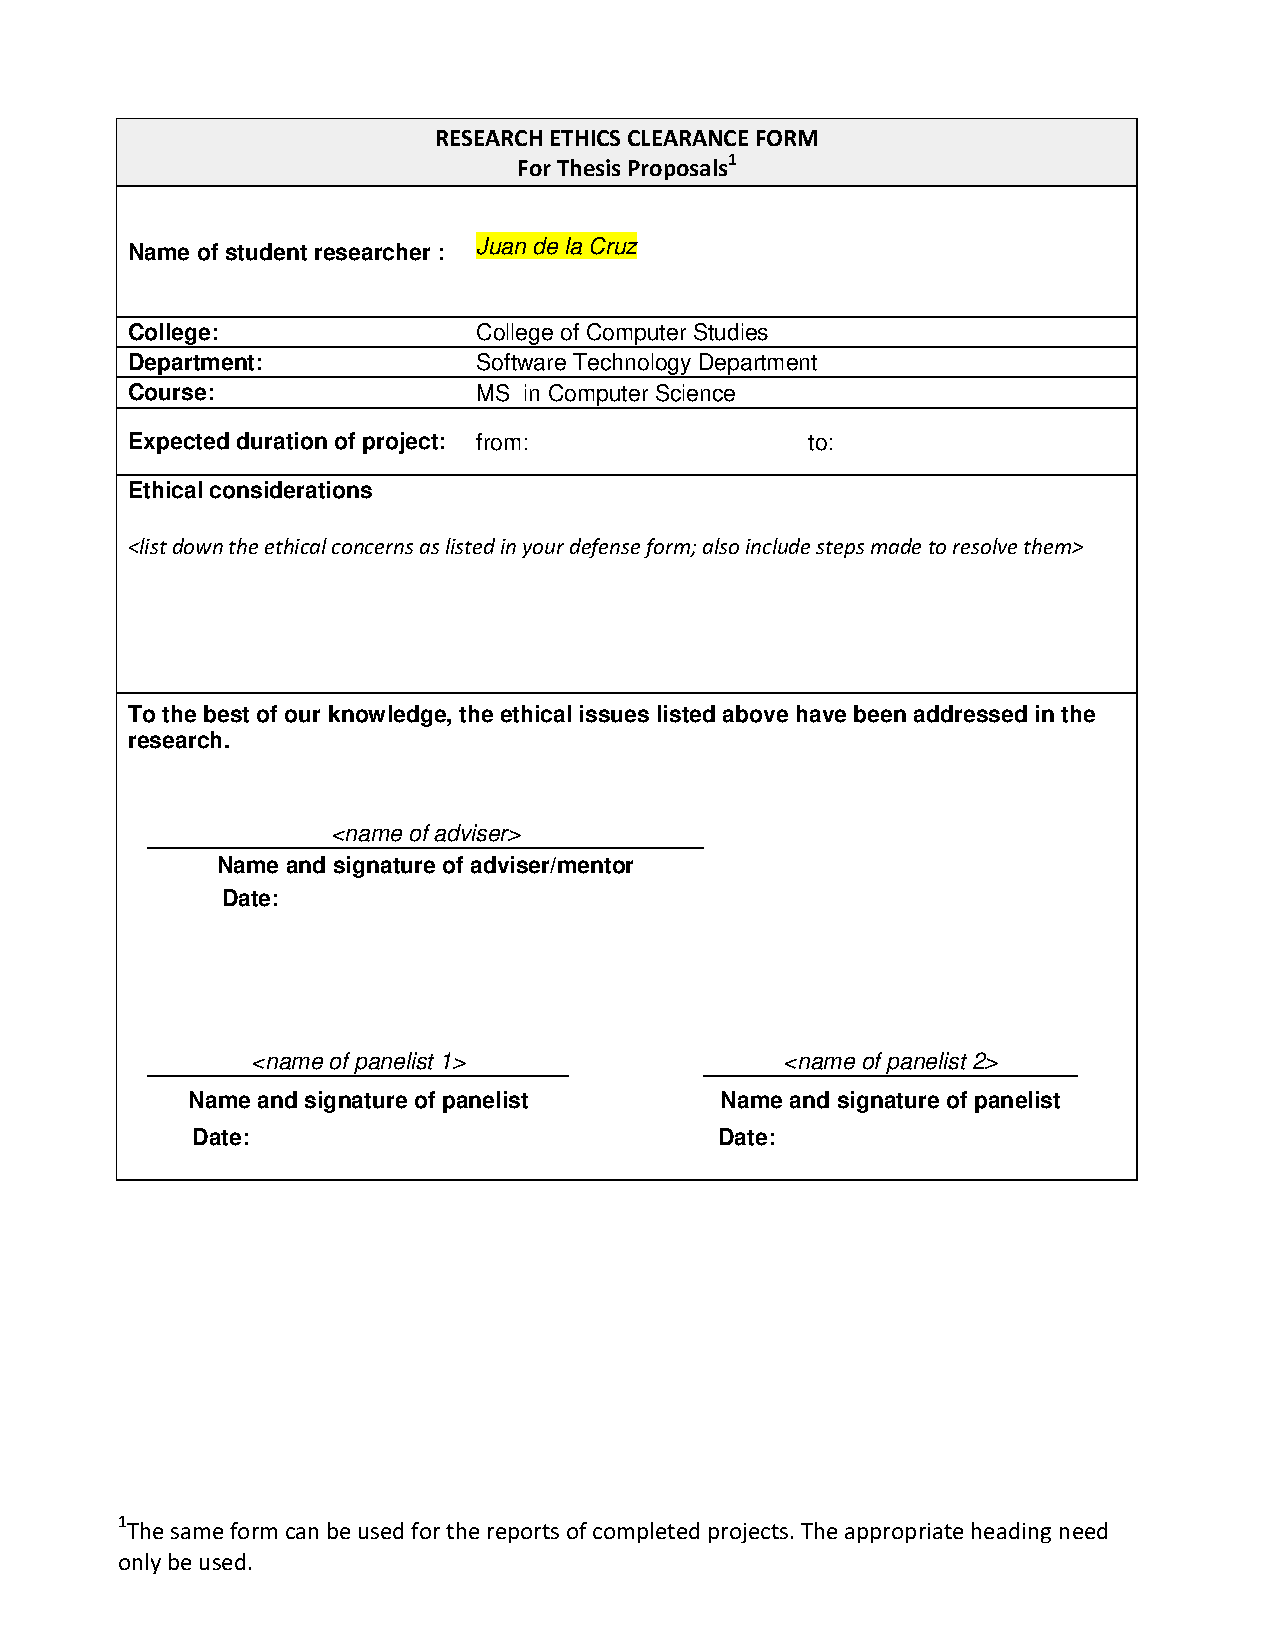
\includepdf[pages=-, scale = 0.9, pagecommand={}, offset = -30 0]{clearance.pdf}

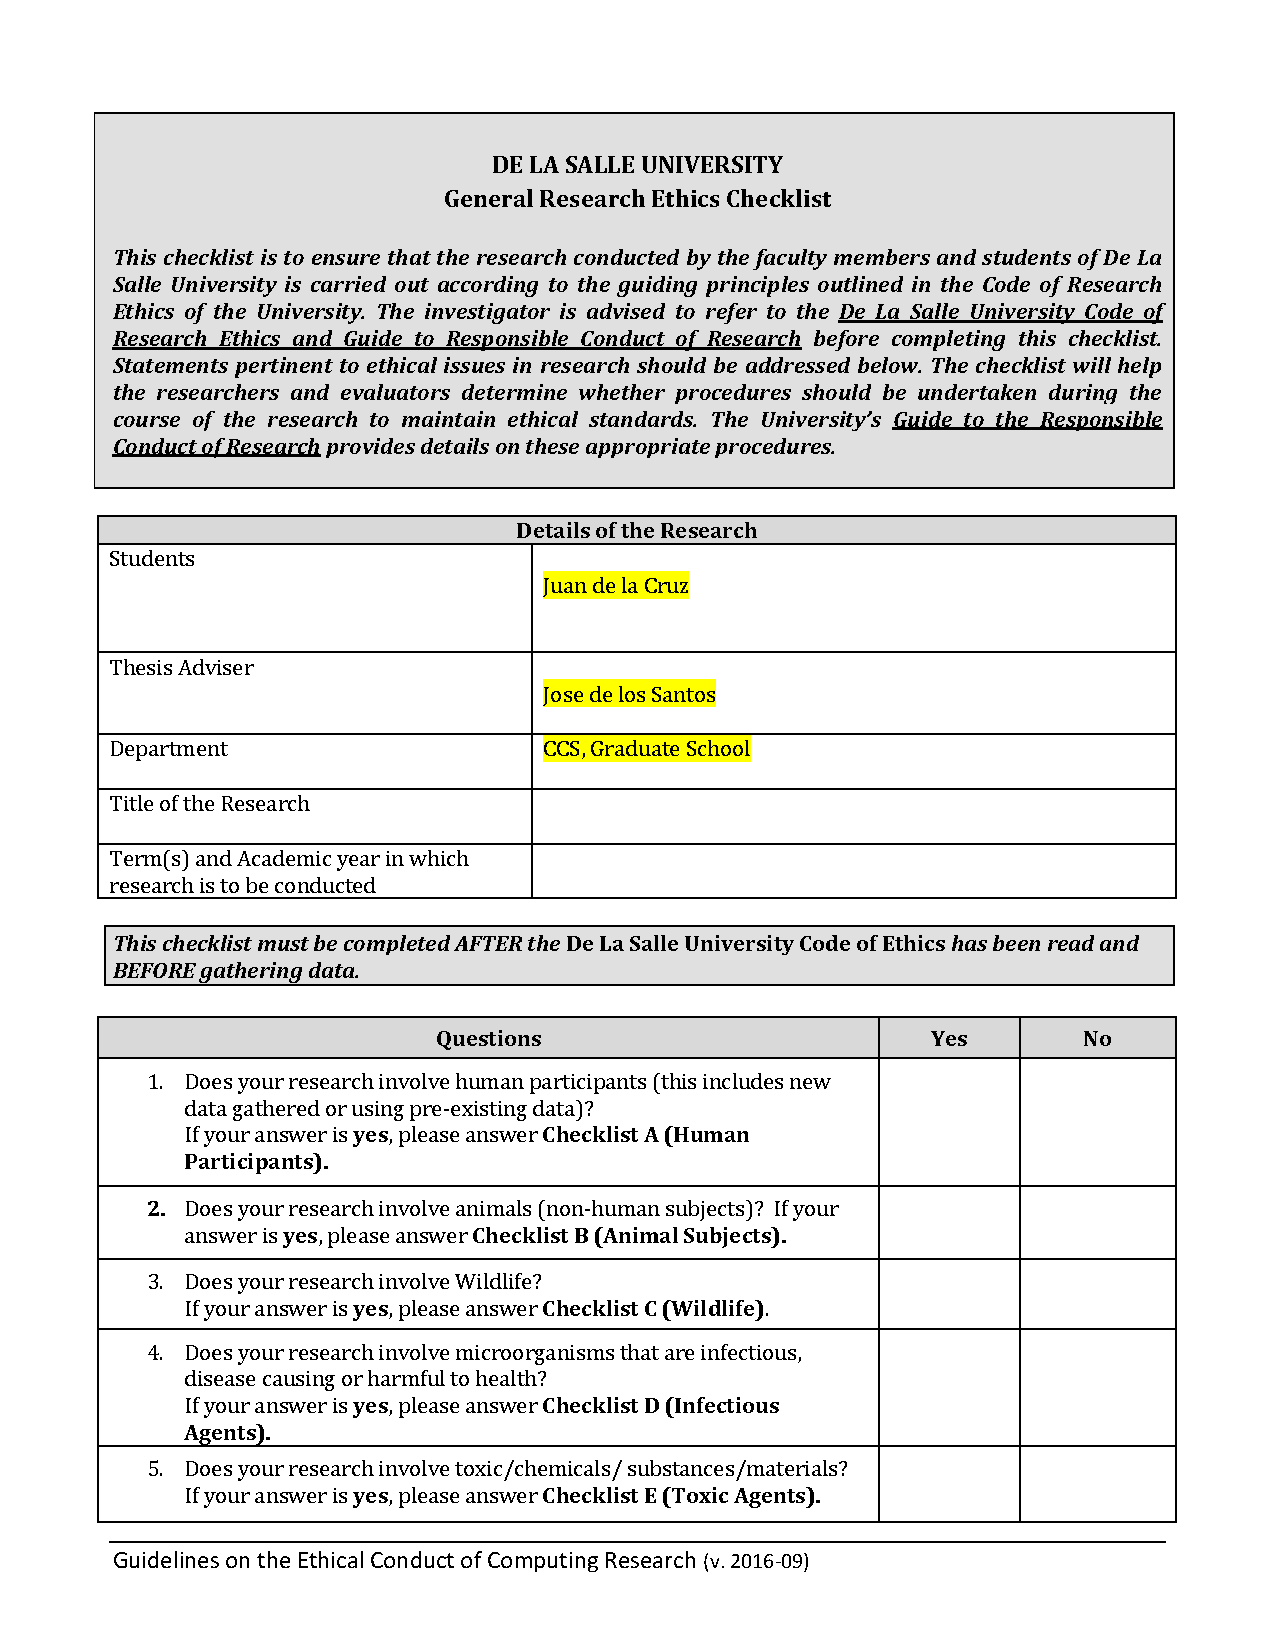
\includepdf[pages=-, scale = 0.9, pagecommand={}, offset = -30 0]{general_checklist.pdf}

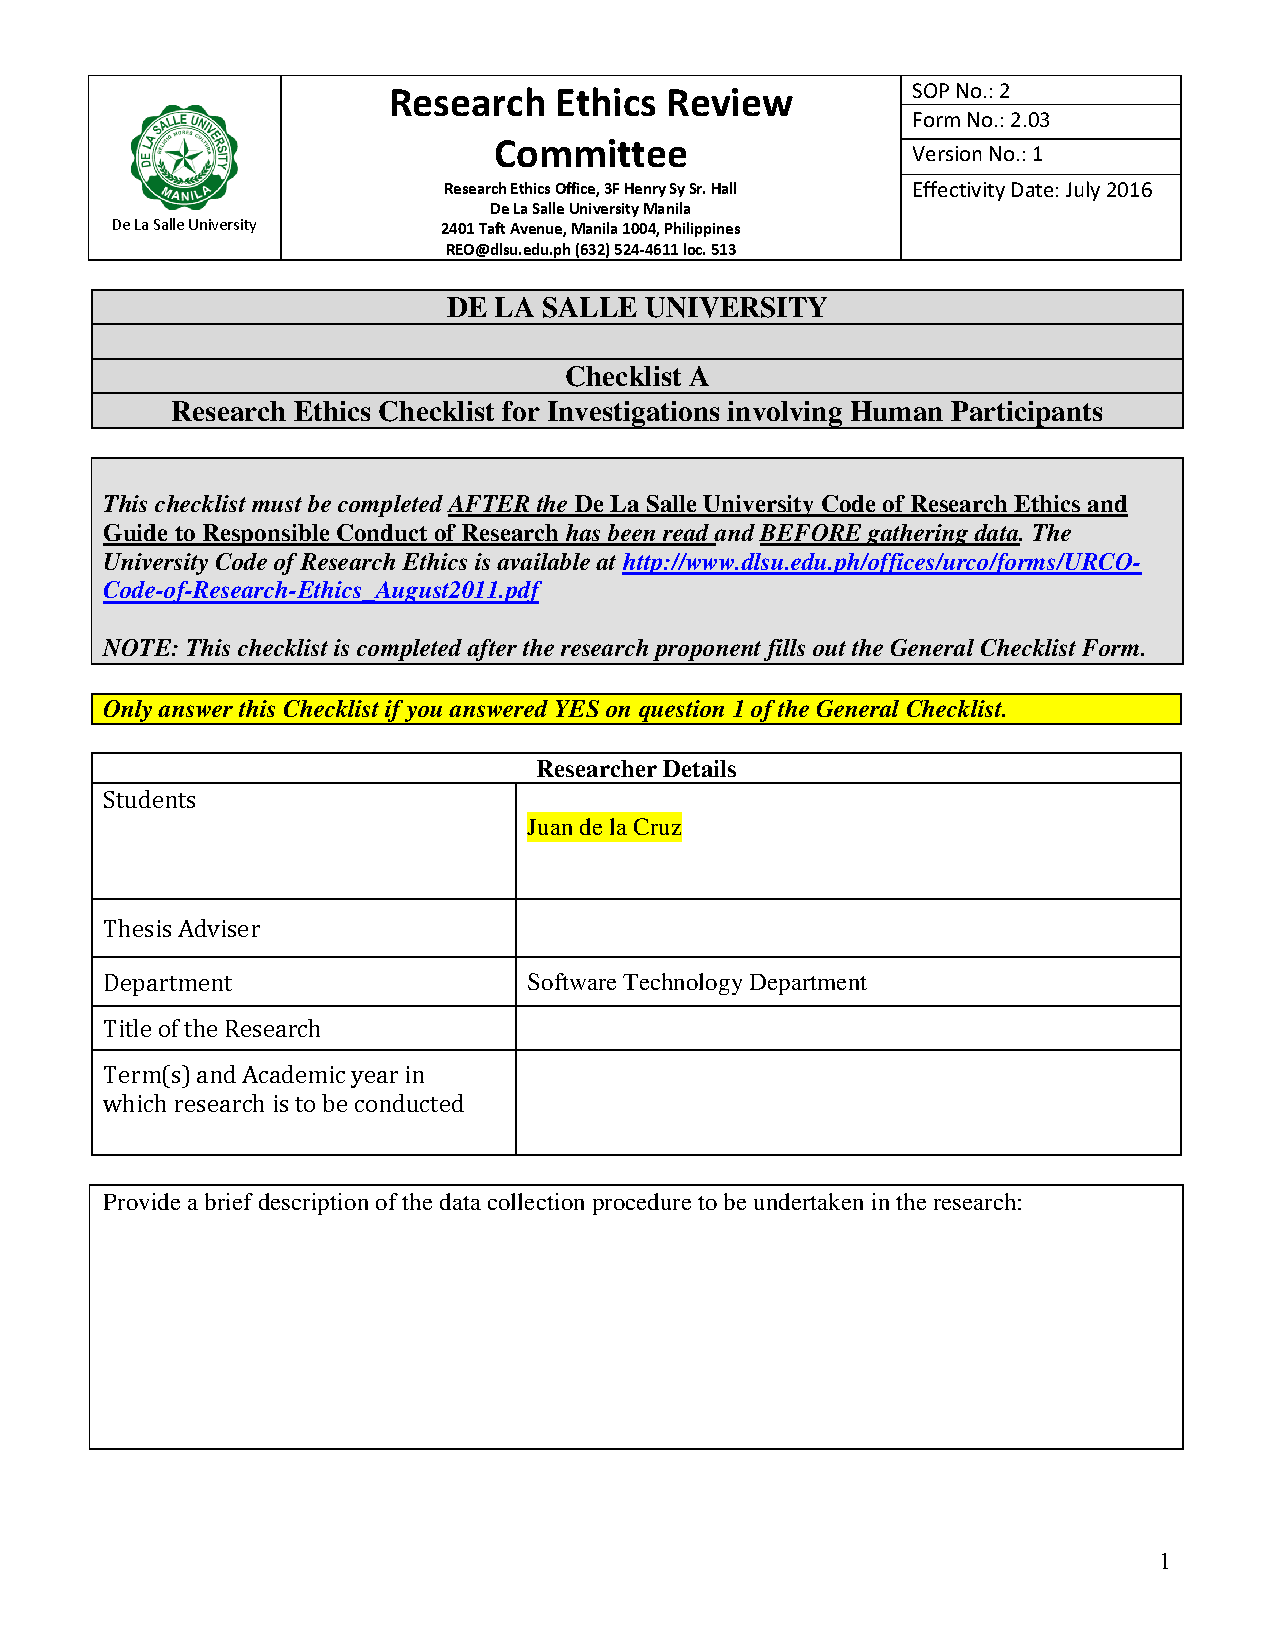
\includepdf[pages=-, scale = 0.9, pagecommand={}, offset = -30 0]{checklist-A.pdf}


